\section{Experiment design}\label{sec:experiment_design}
%Forsoegsopstilling, der inkludere en tegning af omraadet set oppefra med indtegning af beacons, objectern og hvor rigtige position for test person.
Experiments for the evaluation of the implemented system are carried out in an n times n meeting room.
In the room, a partition and a cabinet are placed between two tables, effectively dividing a single meeting room into two smaller areas. 
In each of the smaller areas a table with six chairs is placed and on the walls are placed whiteboards.
\begin{figure}[h]
    \centering
    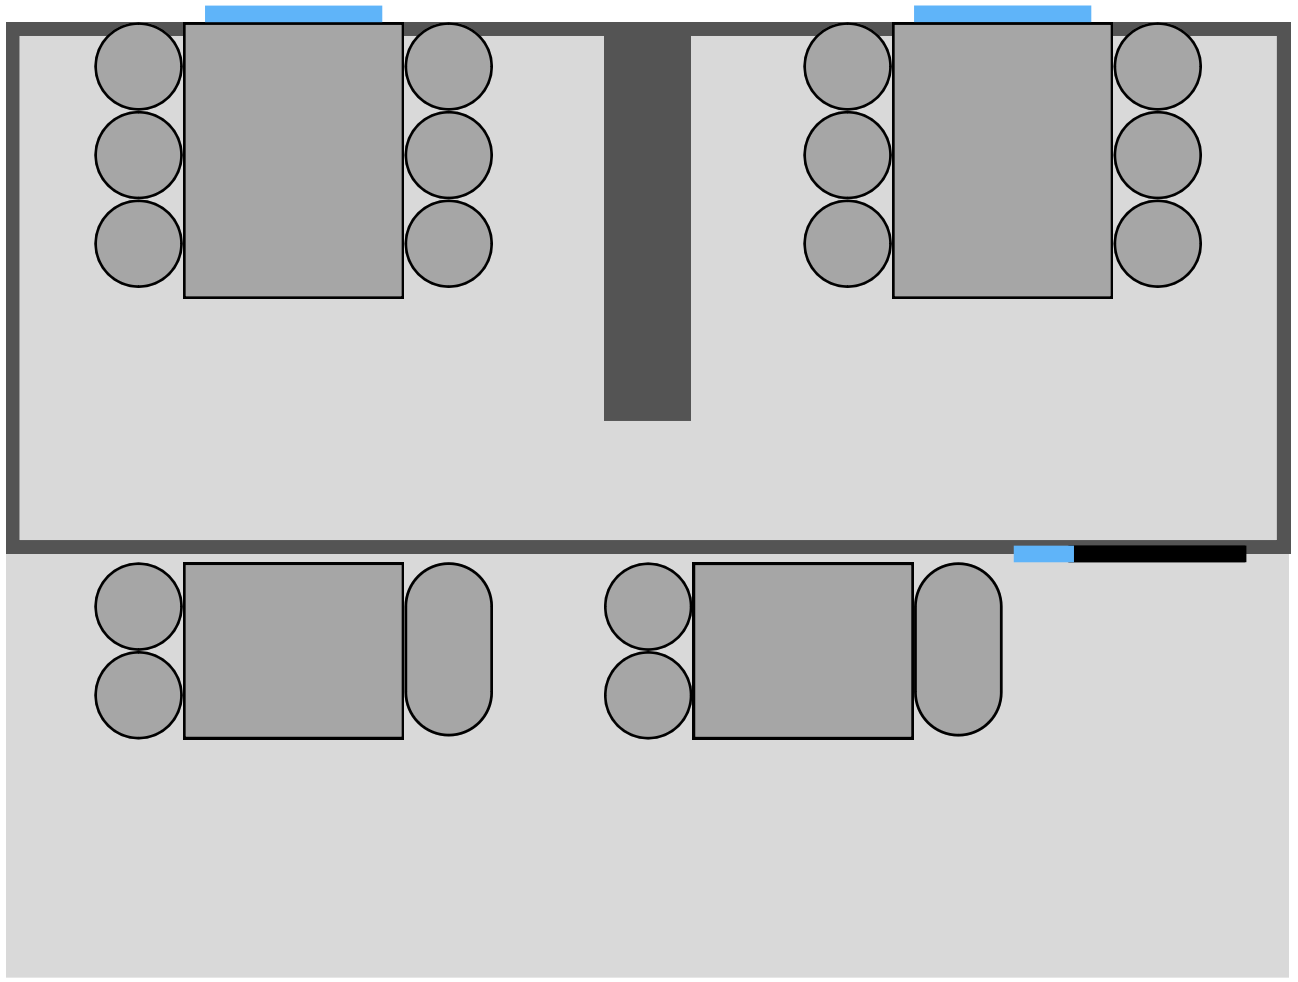
\includegraphics[scale=0.7]{images/experiment_room.png}
    \caption{The meeting room in which the experiments were carried out.}
    \label{fig:experiment_room}
\end{figure}
On one end of each table is a large, rectangular window.
Furthermore, one table has a large TV screen placed near the window. 
Near the door of the room, an airconditioning controller and a large glass window are located.
Lighting is built into the ceiling, thus no hanging light will interfere with the broadcasted signals. 
Outside the meeting room is a common area.
This area contains two high tables.
Each of these tables has a small couch and two chairs placed next to it.   
The meeting room and its surrounding area is depicted in Figure \ref{fig:experiment_room}.

In the room is placed x yyyyy beacons supporting the iBeacon standard~\cite{apple2023ibeacon}.
 


%room description

